% -*- mode: LaTeX; TeX-PDF-mode: t; -*-
% LaTeX path to the root directory of the current project, from the directory in which this file resides
% and path to econtexPaths which defines the rest of the paths like \FigDir
\providecommand{\econtexRoot}{}\renewcommand{\econtexRoot}{.}
\providecommand{\econtexPaths}{}\renewcommand{\econtexPaths}{\econtexRoot/Resources/econtexPaths}
% The \commands below are required to allow sharing of the same base code via Github between TeXLive on a local machine and Overleaf (which is a proxy for "a standard distribution of LaTeX").  This is an ugly solution to the requirement that custom LaTeX packages be accessible, and that Overleaf prohibits symbolic links

\providecommand{\econtex}{\econtexRoot/Resources/texmf-local/tex/latex/econtex}
\providecommand{\pdfsuppressruntime}{\econtexRoot/Resources/texmf-local/tex/latex/pdfsuppressruntime}
\providecommand{\econark}{/Volumes/Sync/GitHub/llorracc/SolvingMicroDSOPs/SolvingMicroDSOPs-Latest/.resources/texmf-local/tex/latex/local-econark}
\providecommand{\econtexSetup}{\econtexRoot/Resources/texmf-local/tex/latex/econtexSetup}
\providecommand{\econtexShortcuts}{\econtexRoot/Resources/texmf-local/tex/latex/econtexShortcuts}
\providecommand{\econtexBibMake}{\econtexRoot/Resources/texmf-local/tex/latex/econtexBibMake}
\providecommand{\econtexBibStyle}{\econtexRoot/Resources/texmf-local/bibtex/bst/econtex}
\providecommand{\econtexBib}{economics}
\providecommand{\economics}{\econtexRoot/Resources/texmf-local/bibtex/bib/economics}
\providecommand{\notes}{\econtexRoot/Resources/texmf-local/tex/latex/handout}
\providecommand{\handoutSetup}{\econtexRoot/Resources/texmf-local/tex/latex/handoutSetup}
\providecommand{\handoutShortcuts}{\econtexRoot/Resources/texmf-local/tex/latex/handoutShortcuts}
\providecommand{\handoutBibMake}{\econtexRoot/Resources/texmf-local/tex/latex/handoutBibMake}
\providecommand{\handoutBibStyle}{\econtexRoot/Resources/texmf-local/bibtex/bst/handout}

\providecommand{\FigDir}{\econtexRoot/Figures}
\providecommand{\CodeDir}{\econtexRoot/Code}
\providecommand{\DataDir}{\econtexRoot/Data}
\providecommand{\SlideDir}{\econtexRoot/Slides}
\providecommand{\TableDir}{\econtexRoot/Tables}
\providecommand{\ApndxDir}{\econtexRoot/Appendices}

\providecommand{\ResourcesDir}{\econtexRoot/Resources}
\providecommand{\rootFromOut}{..} % APFach back to root directory from output-directory
\providecommand{\LaTeXGenerated}{\econtexRoot/LaTeX} % Put generated files in subdirectory
\providecommand{\econtexPaths}{\econtexRoot/Resources/econtexPaths}
\providecommand{\LaTeXInputs}{\econtexRoot/Resources/LaTeXInputs}
\providecommand{\LtxDir}{}
\providecommand{\EqDir}{Equations} % Put generated files in subdirectory

\documentclass[\econtexRoot/BufferStockTheory]{subfiles}
% LaTeX path to the root directory of the current project, from the directory in which this file resides
% and path to econtexPaths which defines the rest of the paths like \FigDir
\providecommand{\econtexRoot}{}\renewcommand{\econtexRoot}{.}
\providecommand{\econtexPaths}{}\renewcommand{\econtexPaths}{\econtexRoot/Resources/econtexPaths}
% The \commands below are required to allow sharing of the same base code via Github between TeXLive on a local machine and Overleaf (which is a proxy for "a standard distribution of LaTeX").  This is an ugly solution to the requirement that custom LaTeX packages be accessible, and that Overleaf prohibits symbolic links

\providecommand{\econtex}{\econtexRoot/Resources/texmf-local/tex/latex/econtex}
\providecommand{\pdfsuppressruntime}{\econtexRoot/Resources/texmf-local/tex/latex/pdfsuppressruntime}
\providecommand{\econark}{/Volumes/Sync/GitHub/llorracc/SolvingMicroDSOPs/SolvingMicroDSOPs-Latest/.resources/texmf-local/tex/latex/local-econark}
\providecommand{\econtexSetup}{\econtexRoot/Resources/texmf-local/tex/latex/econtexSetup}
\providecommand{\econtexShortcuts}{\econtexRoot/Resources/texmf-local/tex/latex/econtexShortcuts}
\providecommand{\econtexBibMake}{\econtexRoot/Resources/texmf-local/tex/latex/econtexBibMake}
\providecommand{\econtexBibStyle}{\econtexRoot/Resources/texmf-local/bibtex/bst/econtex}
\providecommand{\econtexBib}{economics}
\providecommand{\economics}{\econtexRoot/Resources/texmf-local/bibtex/bib/economics}
\providecommand{\notes}{\econtexRoot/Resources/texmf-local/tex/latex/handout}
\providecommand{\handoutSetup}{\econtexRoot/Resources/texmf-local/tex/latex/handoutSetup}
\providecommand{\handoutShortcuts}{\econtexRoot/Resources/texmf-local/tex/latex/handoutShortcuts}
\providecommand{\handoutBibMake}{\econtexRoot/Resources/texmf-local/tex/latex/handoutBibMake}
\providecommand{\handoutBibStyle}{\econtexRoot/Resources/texmf-local/bibtex/bst/handout}

\providecommand{\FigDir}{\econtexRoot/Figures}
\providecommand{\CodeDir}{\econtexRoot/Code}
\providecommand{\DataDir}{\econtexRoot/Data}
\providecommand{\SlideDir}{\econtexRoot/Slides}
\providecommand{\TableDir}{\econtexRoot/Tables}
\providecommand{\ApndxDir}{\econtexRoot/Appendices}

\providecommand{\ResourcesDir}{\econtexRoot/Resources}
\providecommand{\rootFromOut}{..} % APFach back to root directory from output-directory
\providecommand{\LaTeXGenerated}{\econtexRoot/LaTeX} % Put generated files in subdirectory
\providecommand{\econtexPaths}{\econtexRoot/Resources/econtexPaths}
\providecommand{\LaTeXInputs}{\econtexRoot/Resources/LaTeXInputs}
\providecommand{\LtxDir}{}
\providecommand{\EqDir}{Equations} % Put generated files in subdirectory

\onlyinsubfile{% https://tex.stackexchange.com/questions/463699/proper-reference-numbers-with-subfiles
    \csname @ifpackageloaded\endcsname{xr-hyper}{%
      \externaldocument{BufferStockTheory}% xr-hyper in use; optional argument for url of main.pdf for hyperlinks
    }{%
      \externaldocument{BufferStockTheory}% xr in use
    }%
    \renewcommand\labelprefix{}%
    % Initialize the counters via the labels belonging to the main document:
}


\onlyinsubfile{\externaldocument{\LaTeXGenerated/BufferStockTheory}}
\onlyinsubfile{\renewcommand{\LtxDir}{}}

\begin{document}

\hypertarget{ApndxConditionDiagrams}{}

\section{Relational Diagrams for the Inequality Conditions}\label{sec:ApndxConditionDiagrams}

This appendix explains in detail the paper's `inequalities' diagrams (Figures~\ref{fig:RelatePFGICFHWCRICPFFVAC},~\ref{fig:Inequalities}).

\hypertarget{InequalityPFGICFHWCRIC}{}
\begin{figure}
\centering
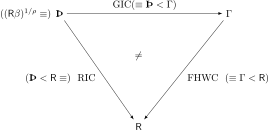
\includegraphics[width=4in]{\FigDir/InequalityPFGICFHWCRIC}
\caption{Appendix: Inequality Conditions for Perfect Foresight Model}
\centerline{ (Start at a node and follow arrows)}\label{fig:InequalityPFGICFHWCRIC}
\end{figure}

\subsection{The Unconstrained Perfect Foresight Model}

A simple illustration is presented in Figure~\ref{fig:InequalityPFGICFHWCRIC}, whose three nodes represent values of the absolute patience factor $\APFac$, the permanent-income growth factor $\PermGroFac$, and the riskfree interest factor $\Rfree$.  The arrows represent imposition of the labeled inequality condition  (like,  the uppermost arrow, pointing from {$\APFac$} to $\PermGroFac$, reflects imposition of the {\GICRaw} condition (clicking {\GICRaw} should take you to its definition; definitions of other conditions are also linked below)).\footnote{For convenience, the equivalent ($\equiv$) mathematical statement of each condition is expressed nearby in parentheses.}  Annotations inside parenthetical expressions containing $\equiv$ are there to make the diagram readable for someone who may not immediately remember terms and definitions from the main text.  (Such a reader might also want to be reminded that $\Rfree, \DiscFac, $ and $\Gamma$ are all in $\mathbb{R}_{++}$, and that $\CRRA>1$).

Navigation of the diagram is simple: Start at any node, and deduce a chain of inequalities by following any arrow that exits that node, and any arrows that exit from successive nodes.  Traversal must stop upon arrival at a node with no exiting arrows.  So, for example, we can start at the $\APFac$ node and impose the {\GICRaw} and then the {\FHWC}, and see that imposition of these conditions allows us to conclude that $\APFac < \Rfree$.

One could also impose $\APFac < \Rfree$ directly (without imposing $\GICRaw$ and $\FHWC$) by following the downward-sloping diagonal arrow exiting $\APFac$.  Although alternate routes from one node to another all justify the same core conclusion ($\APFac < \Rfree$, in this case), $\neq$ symbol in the center is meant to convey that these routes are not identical in other respects.  This notational convention is used in \href{https://en.wikipedia.org/wiki/Diagram_(category_theory)}{category theory diagrams},\footnote{For a popular introduction to category theory, see~\cite{riehl2017category}.} to indicate that the diagram is not \href{https://en.wikipedia.org/wiki/Commutative_diagram}{commutative}.\footnote{But the rest of our notation does not necessarily abide by the other conventions of category theory diagrams.}

Negation of a condition is indicated by the reversal of the corresponding arrow.  For example, negation of the {\RIC},  $\cncl{\RIC} \equiv \APFac > \Rfree$, would be represented by moving the arrowhead from the bottom right to the top left of the line segment connecting {$\APFac$} and $\Rfree$.

If we were to start at $\Rfree$ and then impose $\cncl{\FHWC}$, that would reverse the arrow connecting $\Rfree$ and $\PermGroFac$, but the $\PermGroFac$ node would then have no exiting arrows so no further deductions could be made.  However, if we \textit{also} reversed $\GICRaw$ (that is, if we imposed $\cncl{\GICRaw}$), that would take us to the $\APFac$ node, and we could deduce $\Rfree > \APFac$.  However, we would have to stop traversing the diagram at this point, because the arrow exiting from the $\APFac$ node points back to our starting point, which (if valid) would lead us to the conclusion that $\Rfree > \Rfree$.  Thus, the reversal of the two earlier conditions (imposition of $\cncl{\FHWC}$ and $\cncl{\GICRaw}$) requires us also to reverse the final condition, giving us $\cncl{\RIC}$.\footnote{The corresponding algebra is
\begin{equation}\begin{gathered}\begin{aligned}
  \cncl{\FHWC}:~~~~  \Rfree & < \PermGroFac \notag  
  \\ \cncl{\GICRaw}:~~~~ \PermGroFac & < \APFac %~\left(\equiv (\Rfree \DiscFac)^{1/\CRRA}\right)
                                \label{eq:cnclRIC}
  \\ \Rightarrow \cncl{\RIC}:~~~~\Rfree & < \APFac \notag,
\end{aligned}\end{gathered}\end{equation}.}

Under these conventions, Figure~\ref{fig:RelatePFGICFHWCRICPFFVAC} \hyperlink{RelatePFGICFHWCRICPFFVAC}{in the main text} presents a modified version of the diagram extended to incorporate the {\PFFVAC} (reproduced here for convenient reference).

\ifthenelse{\boolean{Web}}{}{
  \captionsetup[figure]{list=no} % This is just reproducing the earlier figure; don't include it in ToC numbering
  }
\begin{figure}[ht]
  \centerline{
    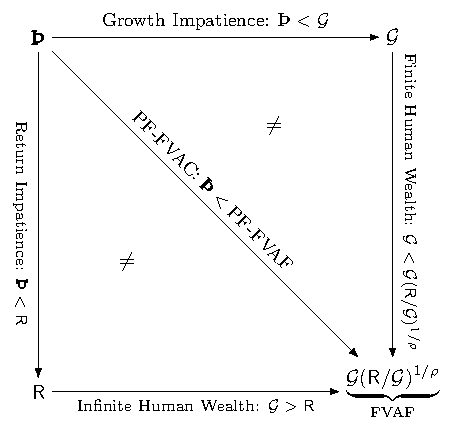
\includegraphics[width=3.5in]{\FigDir/RelatePFGICFHWCRICPFFVAC}
  }
  \caption{Appendix: Relation of {GIC}, {FHWC}, {RIC}, and {PFVAC}}\label{fig:RelatePFGICFHWCRICPFFVACApp}
  \footnotesize{An arrowhead points to the larger of the two quantities being compared.  For example, the diagonal arrow indicates that $\APFac < \Rfree^{1/\CRRA}\PermGroFac^{1-1/\CRRA}$, which is an alternative way of writing the {\PFFVAC},~\eqref{eq:PFFVAC}}
\end{figure}
\ifthenelse{\boolean{Web}}{}{
\captionsetup[figure]{list=yes} % This is just reproducing the earlier figure; don't include it in ToC numbering
}

This diagram can be interpreted, for example, as saying  that, starting at the $\APFac$ node, it is possible to derive the $\PFFVAC$\footnote{in the form $\APFac < {(\Rfree/\PermGroFac)}^{1/\CRRA}\PermGroFac$} by imposing both the {\GICRaw} and the {\FHWC}; or by imposing {\RIC} and \cncl{\FHWC}.  Or, starting at the $\PermGroFac$ node, we can follow the imposition of the {\FHWC} (twice --- reversing the arrow labeled $\cncl{\FHWC}$) and then $\cncl{\RIC}$ to reach the conclusion that $\APFac < \PermGroFac$.  Algebraically,
\begin{equation}\begin{gathered}\begin{aligned}
  {\FHWC}:~~~ \PermGroFac & < \Rfree 
  \\ \cncl{\RIC}:~~~ \Rfree & < \APFac 
  \\ \PermGroFac & < \APFac \label{eq:cnclGICRaw}
\end{aligned}\end{gathered}\end{equation}
which leads to the negation of both of the conditions leading into $\APFac$.  \cncl{\GICRaw} is obtained directly as the last line in~\eqref{eq:cnclGICRaw} and \cncl{\PFFVAC} follows if we start by multiplying the Return Patience Factor ({\RPFacDefn}=$\APFac/\Rfree$) by the {\FHWFacDefn} (=$\PermGroFac/\Rfree$) raised to the power $1/\CRRA-1$, which is negative since we imposed $\CRRA > 1$.  {\FHWC} implies {\FHWFacDefn} $< 1$ so when {\FHWFacDefn} is raised to a negative power the result is greater than one.
Multiplying the {\RPFacDefn} (which exceeds 1 because \cncl{\RIC}) by another number greater than one yields a product that must be greater than one:
\begin{equation}\begin{gathered}\begin{aligned}
  1  & < \overbrace{\left(\frac{{(\Rfree \DiscFac)}^{1/\CRRA}}{\Rfree}\right)}^{>1 \text{~from~}\cncl{\RIC}}\overbrace{{\left(\PermGroFac/\Rfree\right)}^{1/\CRRA-1}}^{\phantom{\ldots}>1~\text{~from~} \FHWC} \notag
  \\ 1  & < \left(\frac{{(\Rfree \DiscFac)}^{1/\CRRA}}{{(\Rfree/\PermGroFac)}^{1/\CRRA}\Rfree\PermGroFac/\Rfree}\right) \label{eq:cnclFHWFacDefnAndcnclRICImplycnclPFFVAC}
  \\ \Rfree^{1/\CRRA}\PermGroFac^{1 - 1/\CRRA} = {(\Rfree/\PermGroFac)}^{1/\CRRA} \PermGroFac  & < \APFac \notag
\end{aligned}\end{gathered}\end{equation}
which is one way of writing $\cncl{\PFFVAC}$.

The complexity of this algebraic calculation illustrates the usefulness of the diagram, in which one merely needs to follow arrows to reach the same result.

After the warmup of constructing these conditions for the perfect foresight case, we can represent the relationships between all the conditions in both the perfect foresight case and the case with uncertainty as shown in Figure~\ref{fig:Inequalities} in the paper (reproduced here).

\begin{figure}[ht]
  \centerline{
    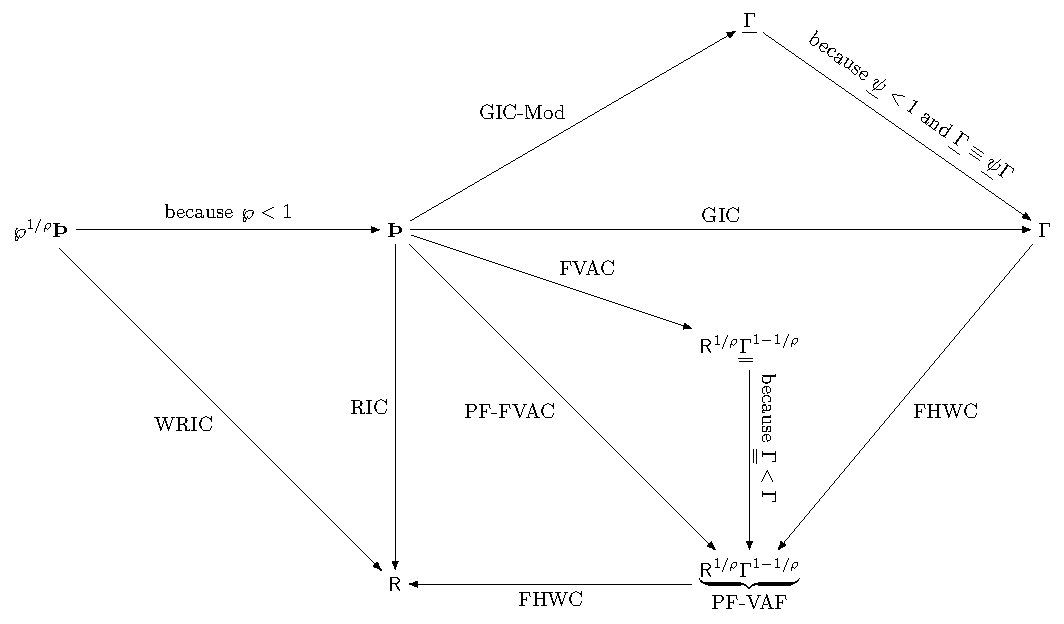
\includegraphics[width=6in]{\FigDir/Inequalities}
  }
  \caption{Appendix: Relation of All Inequality Conditions}\label{fig:InequalitiesApp}
\end{figure}

Finally, the next diagram substitutes the values of the various objects in the diagram under the baseline parameter values and verifies that all of the asserted inequality conditions hold true.
\begin{figure}[ht]
  \centerline{
    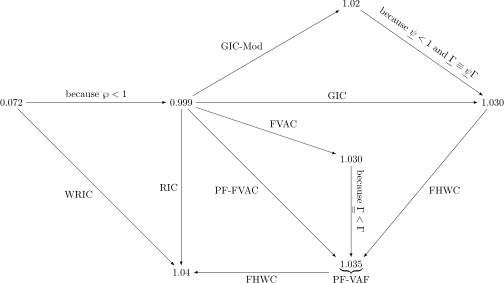
\includegraphics[width=6in]{\FigDir/Inequalities-numer}
  }
  \caption{Appendix: Numerical Relation of All Inequality Conditions}\label{fig:InequalitiesAppNumer}
\end{figure}

%\onlyinsubfile{\bibliography{\LaTeXGenerated/BufferStockTheory,\econtexBib}}
%\onlyinsubfile{\pagebreak\bibliography{\econtexRoot/\texname,\econtexBib}}
\onlyinsubfile{\pagebreak% Allows two (optional) supplements to hard-wired \texname.bib bibfile:
% system.bib is a default bibfile that supplies anything missing elsewhere
% Add-Refs.bib is an override bibfile that supplants anything in \texfile.bib or system.bib
\provideboolean{AddRefsExists}
\provideboolean{systemExists}
\provideboolean{BothExist}
\provideboolean{NeitherExists}
\setboolean{BothExist}{true}
\setboolean{NeitherExists}{true}

\IfFileExists{\econtexRoot/Add-Refs.bib}{
  % then
  \typeout{References in Add-Refs.bib will take precedence over those elsewhere}
  \setboolean{AddRefsExists}{true}
  \setboolean{NeitherExists}{false} % Default is true
}{
  % else
  \setboolean{AddRefsExists}{false} % No added refs exist so defaults will be used
  \setboolean{BothExist}{false}     % Default is that Add-Refs and system.bib both exist
}

% Deal with case where system.bib is found by kpsewhich
\IfFileExists{/usr/local/texlive/texmf-local/bibtex/bib/system.bib}{
  % then
  \typeout{References in system.bib will be used for items not found elsewhere}
  \setboolean{systemExists}{true}
  \setboolean{NeitherExists}{false}
}{
  % else
  \typeout{Found no system database file}
  \setboolean{systemExists}{false}
  \setboolean{BothExist}{false}
}

\ifthenelse{\boolean{showPageHead}}{ %then
  \clearpairofpagestyles % No header for references pages
  }{} % No head has been set to clear

\ifthenelse{\boolean{BothExist}}{
  % then use both
  \typeout{bibliography{\econtexRoot/Add-Refs,\econtexRoot/\texname,system}}
  \bibliography{\econtexRoot/Add-Refs,\econtexRoot/\texname,system}
  % else both do not exist
}{ % maybe neither does?
  \ifthenelse{\boolean{NeitherExists}}{
    \typeout{bibliography{\texname}}
    \bibliography{\texname}}{
    % no -- at least one exists
    \ifthenelse{\boolean{AddRefsExists}}{
      \typeout{bibliography{\econtexRoot/Add-Refs,\econtexRoot/\texname}}
      \bibliography{\econtexRoot/Add-Refs,\econtexRoot/\texname}}{
      \typeout{bibliography{\econtexRoot/\texname,system}}
      \bibliography{        \econtexRoot/\texname,system}}
  } % end of picking the one that exists
} % end of testing whether neither exists
}

\end{document}
\endinput


% Local Variables:
% eval: (setq TeX-command-list  (assq-delete-all (car (assoc "BibTeX" TeX-command-list)) TeX-command-list))
% eval: (setq TeX-command-list  (assq-delete-all (car (assoc "BibTeX" TeX-command-list)) TeX-command-list))
% eval: (setq TeX-command-list  (assq-delete-all (car (assoc "BibTeX" TeX-command-list)) TeX-command-list))
% eval: (setq TeX-command-list  (assq-delete-all (car (assoc "BibTeX" TeX-command-list)) TeX-command-list))
% eval: (setq TeX-command-list  (assq-delete-all (car (assoc "Biber"  TeX-command-list)) TeX-command-list))
% eval: (setq TeX-command-list  (remove '("BibTeX" "%(bibtex) LaTeX/%s"    TeX-run-BibTeX nil t :help "Run BibTeX") TeX-command-list))
% eval: (setq TeX-command-list  (remove '("BibTeX" "bibtex LaTeX/%s"    TeX-run-BibTeX nil t :help "Run BibTeX") TeX-command-list))
% eval: (add-to-list 'TeX-command-list '("BibTeX" "bibtex ../LaTeX/%s" TeX-run-BibTeX nil t                                                                              :help "Run BibTeX") t)
% eval: (add-to-list 'TeX-command-list '("BibTeX" "bibtex ../LaTeX/%s" TeX-run-BibTeX nil (plain-tex-mode latex-mode doctex-mode ams-tex-mode texinfo-mode context-mode) :help "Run BibTeX") t)
% TeX-PDF-mode: t
% TeX-file-line-error: t
% TeX-debug-warnings: t
% LaTeX-command-style: (("" "%(PDF)%(latex) %(file-line-error) %(extraopts) -output-directory=../LaTeX %S%(PDFout)"))
% TeX-source-correlate-mode: t
% TeX-parse-self: t
% eval: (cond ((string-equal system-type "darwin") (progn (setq TeX-view-program-list '(("Skim" "/Applications/Skim.app/Contents/SharedSupport/displayline -b %n ../LaTeX/%o %b"))))))
% eval: (cond ((string-equal system-type "gnu/linux") (progn (setq TeX-view-program-list '(("Evince" "evince --page-index=%(outpage) ../LaTeX/%o"))))))
% eval: (cond ((string-equal system-type "gnu/linux") (progn (setq TeX-view-program-selection '((output-pdf "Evince"))))))
% TeX-parse-all-errors: t
% End:
